\documentclass[
  twoside,
  12pt, a4paper,
  footinclude=true,
  headinclude=true,
  cleardoublepage=empty
]{scrbook}

\usepackage{lipsum}
\usepackage[italian, english]{babel}
\usepackage[linedheaders,parts,pdfspacing]{classicthesis}
\usepackage{graphics,color}
\usepackage{newlfont}
\usepackage{amssymb}
\usepackage{amsmath}
\usepackage{latexsym}
\usepackage{amsthm}
\usepackage{float}
\usepackage[dvips]{graphicx}
\usepackage{graphicx}
\usepackage{indentfirst}
\usepackage{mathtools}
\usepackage{eurosym}
\usepackage{acronym}
\usepackage[sans]{frontespizio}

\hyphenation{}                                                                                

\newtheorem{theorem}{Theorem}[section]                                  
\newtheorem{proposition}[theorem]{Proposition}                         
\newtheorem{corollary}[theorem]{Corollary}                                 
\newtheorem{lemma}[theorem]{Lemma}                                        
\theoremstyle{definition}               
\newtheorem{definition}[theorem]{Definition}                               
\newtheorem{osse}[theorem]{Osservazione}                                
\newtheorem{example}{Example}[section]                                     

\begin{document}

\frontmatter

\begin{frontespizio}
\Istituzione{\textsc{\LARGE Universit\'a del Salento}}
\Logo[3cm]{salento}
\Facolta{\textsc{Scienze Matematiche, Fisiche e Naturali}}
\Corso{Matematica}
\Annoaccademico{2014--2015}
\Titoletto{\large{\bf Tesi di Laurea Magistrale in \\
Algoritmi e Complessit\'a}}
\Titolo{Thesis Title}
\Rientro{2cm}
\Candidato[20015127]{Roberta Monteforte}
\Relatore{Antonio Caruso}
\end{frontespizio}

\include{FrontBackMatter/abstract}
\include{FrontBackMatter/dedication}
\include{FrontBackMatter/acknowledgements}
\include{FrontBackMatter/declaration}
\include{FrontBackMatter/contents}

\mainmatter

\part{First Part of My Thesis}

\chapter{Modeling the Line Planning Problem}

\section{Preliminary Definition}
In this section, we will identify the basic ingredients of the Line Planning Problem.
\begin{definition}
A PTN=(V, E) is an undirected network. It represents a public tranportation network with stops (or station) V and physical connections (i.e. the tracks) E.
\end{definition}
The PTN describes the underlying street or track network we assume to be given and fixed. We assume that all lines will be operated by homogeneous vehicles, i.e., we only consider one single transport mode. In particular, we are going to consider buses. This is certainly not a realistic assumption, but nevertheless makes algorithmically sense since different modes of transport are often considered one after another.
\begin{definition}
A \textbf{line} is a path in the PTN which is served by buses. 
\begin{itemize}
\item A \textbf{one-directional line} l is given by a sequence (s$_1$, e$_1$, s$_2$, e$_2$, ..., e$_{k-1}$, s$_k$) of vertices s$_i$ $\in$ S and edges e$_i$ $\in$ E such that e$_i$ = \{s$_i$, s$_{i+1}$\} which contains every node of the PTN at most once, unless s$_1$ = s$_k$.
\item A \textbf{bi-directional line} is a sequence (s$_1$, e$_1$, s$_2$, e$_2$, ..., e$_{k-1}$, s$_k$, e$_{k-1}$, e$_2$, s$_2$, e$_1$, s$_1$) with s$_i$ $\ne$ s$_j$ for all i, j.
\end{itemize}
\end{definition}
Every line l is assigned a monotonously increasing function $\alpha_l$ : $\mathbb{R}^+_0 \rightarrow \mathbb{R}^0_+$, called \textbf{line driving time function}. \newline
Furthermore, every line is assigned a line cost $\beta_l$ which specifies the ost caused by establishing line l with frequency f$_l$. The line cost $\beta_l$ consists of a fixed cost $\kappa$ $\ge$ 0 and a per-bus cost b$_l$ > 0, i.e. $\beta_l$(f$_l$) = b$_l$f$_l$ + $\kappa_l$. \newline
We denote by:
\begin{itemize}
\item S(l) := \{s $\in$ S: s $\in$ l\} the stations visited by line l
\item E(l) := \{e $\in$ E: e $\in$ l\} the edges visited by line l
\item $\mathcal{L}$(s) := \{l: l $\ni$ s\} the lines visiting a given station s
\item $\mathcal{L}$(e) := \{l: l $\ni$ e\} the lines visiting a given edge e
\end{itemize}
\begin{definition}
A \textbf{line pool} $\mathcal{L}$ is a set of lines from which the lines can be choosen.
\end{definition}
\begin{definition}
The \textbf{frequency} f$_l$ $\in$ $\mathbb{N}$ of a line l says how often service is offered along line l within a given time period. 
\end{definition}
In capacited line planning, a \textbf{line concept} is  set $\mathcal{L'}$ $\subset$ $\mathcal{L}$ together with a frequency f$_l$  $\in$ for every l $\in$ $\mathcal{L'}$. Since in uncapacited line planning the frequencies are either 0 (the line is not contained in the line concept) or 1 (the line is contained in the line concept), we often omit stating the frequencies explicitly and call $\mathcal{L'}$ a line concept. \newline
We assume an overall budget B on the costs of a line concept. That is, a line concept $\mathcal{L'}$ $\subset$ $\mathcal{L}$ is \textbf{feasible} if $\sum_{l\in\mathcal{L'}}$ $\beta_l$ $\le$ B. 
The passengers' demand for traveling between the station is given by the OD-pairs set.
\begin{definition}
A set of \textbf{OD-pairs} is a subset of pairs of station $\mathcal{OD}$ = \{(u$_i$, v$_i$): i = 1,...,m\} $\subset$ S $\times$ S. There is a weight w$_{uv}$ assigned to each OD-pair representing the number of passengers who want to travel from s(u) to s(v).
\end{definition}
In order to describe a passenger's journey, we now introduce the following important definition.
\begin{definition}
A \textbf{line-route} P$_{uv}$ for a passenger of OD-pair (u, v) $\in$ $\mathcal{OD}$ specifies
\begin{itemize}
\item a path P = (s$_1$, e$_1$, s$_2$, e$_2$, ..., e$_{j-1}$, s$_j$) with s$_1$ := u and s$_j$ := v
\item for each edge e$_i$ $\in$ P a line l $\in$ P a line l $\in$ $\mathcal{L}$(e$_i$) which is chosen for traveling on e$_i$
\end{itemize}
P is called the \textbf{path corresponding to} P$_{uv}$ in the PTN. Moreover, we say that a line-route P$_{uv}$ is \textbf{feasible} for a line concept $\mathcal{L'}$ if P$_{uv}$  uses only lines contained in $\mathcal{L'}$. Note that P$_{uv}$ does not only specify the path in the PTN, but also the lines used for traveling on the path and the stations whare transfers between lines take place.
\end{definition}
The travel time along P$_{uv}$ includes the riding time and a penalty for every transfer:
\begin{equation} \notag
c(\mathcal{L'}, P) := d(\mathcal{L'}, P) + t(\mathcal{L'}, P)
\end{equation}
where
\begin{itemize}
\item d($\mathcal{L'}$, P) = $\sum_{e \in P}$ $\alpha_l$L$_e$, with L$_e$ edge lenght, is the driving time
\item t($\mathcal{L'}$, P) =  $\sum_{s \in P} p^{ll'}_s$, is the transfer time. We observe that the trasfer penalties $p^{ll'}_s$ are assumed to depend on the station s where the transfer takes place and on the lines l and l' between it is performed.
\end{itemize}
\begin{definition} A \textbf{line-routing for OD-pair (u, v)} is a set $\mathcal{R}_{uv}$:= \{P: line-route P is used by (u, v)\} that specifies a line-route for every passenger in (u, v). \newline
A \textbf{line-routing} $\mathcal{R}$ is a set which contains a line-routing for every OD-pair (u, v) $\in$ $\mathcal{OD}$:
\begin{equation} \notag
\mathcal{R} := \{P_{uv} : (u, v) \in \mathcal{OD}\}
\end{equation}
\end{definition}
We denote by w$^P_{uv}$ the number of passengers of OD-pair (u, v) using the line route P and require that $\sum_{P \in \mathcal{R}_{uv}}$ w$^P_{uv}$ = w$_{uv}$. In uncapacited line planning we assume that all passengers of n OD-pair take the same line-route and, in this case a line-routing is just a collection of exactly one path p$_{uv}$ for every OD-pair (u, v). \newline
A line-routing $\mathcal{R}$ is \emph{feasible for a given line concept} $\mathcal{L'}$ if every line-route in $\mathcal{R}$ is feasible for $\mathcal{L'}$ . \newline
On the other hand, a line concept $\mathcal{L'}$ is \emph{feasible for a line-routing} $\mathcal{R}$ if it is a feasible line-concept, if all lines used by $\mathcal{R}$ are contained in $\mathcal{L'}$. \newline
Obviously both these definitions require additional constraints in case of capacity restrictions. \newline
Let $\mathcal{L'}$ be a line concept and $\mathcal{R}$ a line-routing. The \emph{overall travel time} is defined as
\begin{equation} \notag
c(\mathcal{L'}, \mathcal{R}) := \sum_{(u, v) \in \mathcal{OD}} \sum_{P \in \mathcal{R}_{uv}} w^P_{uv}c(\mathcal{L'}, P)
\end{equation} 

\section{The Change-and-Go Network}
In order to depict the various travel possibilities from the origins to the destinations, we introduce the change-and-go network (CGN). The concept of the change-and go network combines the PTN, the line pool and the OD-pairs into one network model. \newline 
Given a public transportation network $\mathcal{PTN}$ = (S, E), a line pool $\mathcal{L}$ and a set of OD-pairs $\mathcal{OD}$, the CGN = (V, A) is constructed in the following way. \newline
The set of nodes V is defined as
\begin{equation} \notag
V := V_{travel} \cup V_{org} \cup V_{dest}
\end{equation}
where
\begin{itemize}
\item V$_{travel}$ := \{[s, l] : s $\in$ S, l $\in$ $\mathcal{L}$(s)\} is the set of \emph{travel nodes}
\item V$_{org}$ := org($\mathcal{OD}$) = \{u$^{org}$ : (u, v) $\in$ $\mathcal{OD}$\} is the set of \emph{origin nodes}
\item V$_{dest}$ := dest($\mathcal{OD}$) := \{v$^{dest}$ : (u, v) $\in$ $\mathcal{OD}$\} is the set of \emph{destination nodes}
\end{itemize}
In these definitions, org and dest are two mapping that map an OD-pair (u, v) to an \emph{origin node} u$^{org}$ := org(u, v) and to a \emph{destination node} v$^{dest}$ := dest(u, v). \newline
The edge set A is defined as
\begin{equation} \notag
A := A_{drive} \cup A_{trans} \cup A_{org} \cup A_{dest}
\end{equation}
where
\begin{itemize}
\item A$_{drive}$ := \{([s, l], [s', l]) : l $\in$ $\mathcal{L}$, \{s, s'\} $\in$ E(l), s$\le_{l}$ s'\} $\subset$ V$_{travel}$ x V$_{travel}$ is the set of \emph{driving arcs}. The lenght of a driving arc ([s, l], [s', l]) is given as c$_{([s, l], [s', l])}$ := L$^l_{ss'}$
\item A$_{trans}$ := \{([s, l], [s, l']) : s $\in$ S, l $\ne$ l' $\in$ $\mathcal{L}$(s)\} $\subset$ V$_{travel}$ x V$_{travel}$ is the set of \emph{tranfer arcs}. The lenght of a transfer arc ([s, l], [s, l'])  is given as c$_{([s, l], [s, l'])}$ := p$^{ll'}_s$
\item A$_{org}$ := \{(u$^{org}$, [u, l]) : u$^{org}$ $\in$  V$_{org}$, [u, l] $\in$ V$_{travel}$\} is the set of \emph{origin arcs} $\subset$ V$_{org}$ x V$_{travel}$. The lenght of every origin arc (u$^{org}$, [u, l]) is set to c$_{(u^{org}, [u, l])}$ := 0
\item A$_{org}$ := \{([v, l], v$^{dest}$) : v$^{dest}$ $\in$  V$_{dest}$, [v, l] $\in$ V$_{travel}$\} is the set of \emph{destination arcs} $\subset$ V$_{travel}$ x V$_{dest}$. The lenght of every destination arc ([v, l], v$^{dest}$) is set to c$_{([v, l], v^{dest})}$ := 0
\end{itemize} 
The following is an example on the onstruction of the CGN.\newline
In Figure 1 is depicted the public transportation network. The nodes represent stations, the edges represent possible direct rides.\newline
The line pool is $\mathcal{L}$ = \{l$_1$ : A - B - C, l$_2$ : D - E - F, l$_3$: A - D - E - B - A, l$_4$: C - F\} with line-driving time $\alpha_{l_1}$(x) := $\frac{1}{2}$x, $\alpha_{l_2}$(x) := $\frac{1}{3}$x, $\alpha_{l_3}$(x) := x and $\alpha_{l_4}$ := $\frac{5}{4}$x. The OD-pairs are (A, F) and (D, C). \newline
\begin{figure}[htbp]
\centering
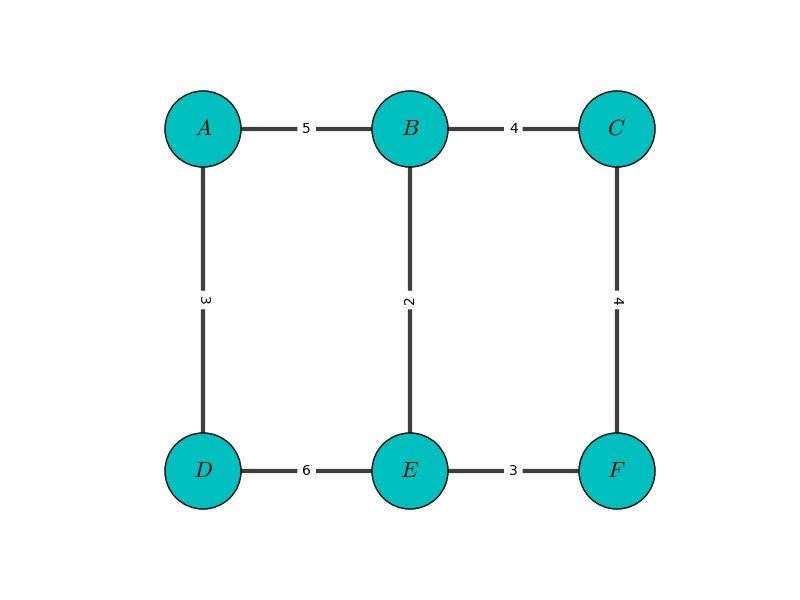
\includegraphics[width=10cm]{esempio1.jpeg}% 
\caption{Public transportation network}
\end{figure}
In Figure 2 the CGN is shown. The yellow lines represent the origins and destinations of the passengers and the green lines stand for the transfer possibilities between two lines.\newline
\begin{figure}[htbp]
\centering
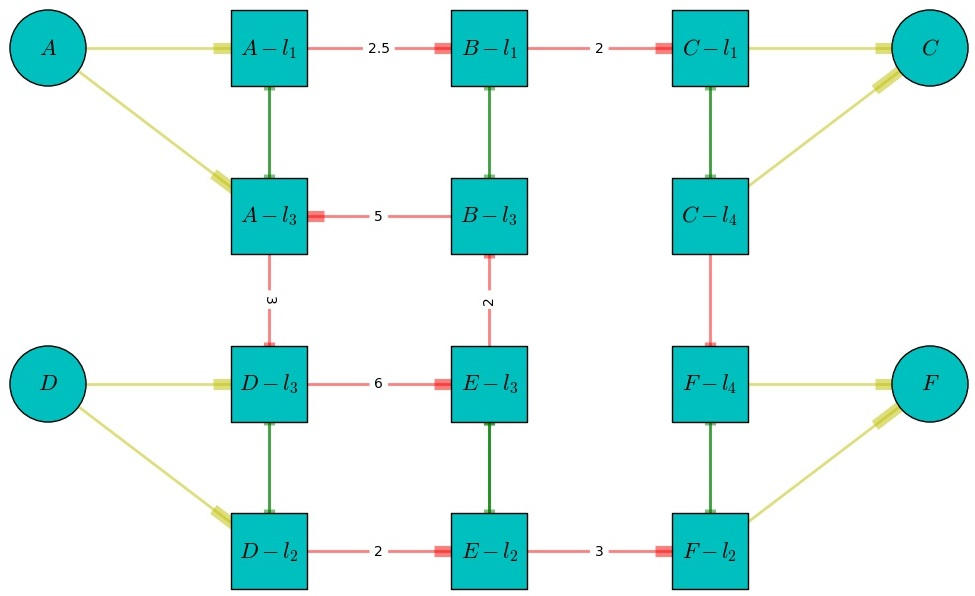
\includegraphics[width=12cm]{figura1.jpg}% 
\caption{Constructed change\&go network}
\end{figure}

\chapter{Solving uncapacited line planning with an extended OD-pairs set}
\section{Problem description}
In this section we assume the following situation: \newline
from a pre-existing line concept $\mathcal{L'}$, the transportation management company wants to expand the set of OD-pairs to satisfy a growing demand. \newline
The transportation company wants to satisfy the demand, but also alter the line concept $\mathcal{L'}$ as little as possible. In fact, it is often important that the established line concept is preserved so as not to jeopardize relationships with current passenger and as to avoid high costs of line concept's modification. As any changes to the transit system must be commensurate with budgetary resources, in many cases the planners are not in the position to accept the most desiderable solution and they have to prioritize any modifications in order to best use available resources. \newline
Let be $\mathcal{OD'}$ = $\mathcal{OD}\cup$\{(u$_i$, v$_i$): i=m,...,t\} the new OD-pairs set.
\begin{definition} An instance ($\mathcal{PTN}$, $\mathcal{L}$, $\mathcal{L'}$, $\mathcal{OD'}$, B') of \emph{uncapacited line planning with an extended OD-pairs set} consists of a public transportation network $\mathcal{PTN}$, a line pool $\mathcal{L}$, the line concept $\mathcal{L'}$ (i.e. the solution of the problem ($\mathcal{PTN}$, $\mathcal{L}$, $\mathcal{OD}$, B)), a set of OD-pairs $\mathcal{OD'}$ and a budget B'. \newline
The task is to choose a feasible line concept $\mathcal{L''}$ and a feasible line-routing $\mathcal{R'}$, such that the overall travel time c($\mathcal{L''}$, $\mathcal{R'}$) of the passenger is minimized while the line concept $\mathcal{L''}$ is as much similar as possible to the line concept $\mathcal{L'}$. 
\end{definition}
In order to preserve the existing line-concept without significantly decrease the quality of the service for passengers, the problem can be modeled as:
\begin{enumerate}
\item the previous line planning problem with routing, in which we are going to introduce a new line pool that take into account the new requirements
\item a bi-criteria optimization problem
\end{enumerate}
In the following sections we analyze the different approaches.
\section{First approach}
In this first approach, we want to use the objective function of the original model's formulation and model the new situation by modifing the line pool $\mathcal{L'}$. \newline
We firstly observe that, in the original problem formulation, it didn't specify how the line pool $\mathcal{L}$ is built. We can reasonably assume that the line pool is constructed by generating for each pair of terminals (s(u), s(v)) all lines whose  travel time is less than or equal to k-times the travel time of the shortest path between s(u) and s(v). \newline
In order to encourage the use of the lines already existing in $\mathcal{L'}$, we add to the line pool $\mathcal{L}$ the set of lines, $\mathcal{S}$, constructed in the following way. Let be
\begin{equation} \notag
p^l_{ij} := \eta c^l_{ij} \quad \quad \forall (i, j) \in E(l), \quad \forall l \in \mathcal{L'}
\end{equation}
where $\eta$ is a proportionality factor, 0 $\le$ $\eta$ $\le$ 1. \newline
Thus, we consider a new PTN that differs from the original only for the driving time p$^l_{ij}$ of line in $\mathcal{L'}$. The set $\mathcal{S}$ is then constructed in the same way of $\mathcal{L}$, but using the new PTN. By now, we consider as line pool the set 
\begin{equation} \notag
n\mathcal{L} = \mathcal{L} \cup \mathcal{S}
\end{equation}
Obviously, the new driving time on the edges in the lines in $\mathcal{L'}$ influence the optimization process; in fact:
\begin{itemize}
\item if 0 $\le$ $\eta$ < 1, then p$^l_{ij}$ < c$^l_{ij}$. In this case the passengers consider more time-effective use the edge in a line in the line concept $\mathcal{L'}$ than in a new line
\item if $\eta$ = 1, then p$^l_{ij}$ = c$^l_{ij}$ and the passengers correctly evaluate the driving time of the edge
\end{itemize}
We have to analyze the cost of building or modifying a line l. Let be $\delta$ the cost of building a detour from a line in $\mathcal{L'}$. Thus: 
\[b'_l=
\begin{cases}
0 &  l \in \mathcal{L'}\\
b_l & l \notin \mathcal{L'}\\
n_l\delta & E(l')\subset E(l), l'\in\mathcal{L'}
\end{cases}
\]
where n$_l$ := \#\{(i, j) : (i, j) $\in$ E(l) $\setminus$ E(l')\}. \newline
Therefore the uncapacited line planning problem with an extended OD-pairs set is a simple uncapacited line planning problem with instance ($\mathcal{PTN}$, n$\mathcal{L}$, $\mathcal{OD'}$, B'). So our objective is 
\begin{equation} \notag
min \sum_{(u,v)\in\mathcal{OD'}} w_{uv}W(s(u), s(v))
\end{equation}
\begin{equation} \notag
s.t. \sum_{l\in\mathcal{L''}} b'_l \le B'
\end{equation}
Obviously, for construction, we aspect that for the OD-pairs in $\mathcal{OD}$ will be chosen the lines in $\mathcal{L'}$, while the parameter $\eta$ and the budget B' are crucial for the re-use of the line in the previous line-concept  for the new OD-pairs.
\section{Second approach} 
The uncapacited line planning problem with an extended OD-pairs set is not only passenger-oriented, but also cost-oriented. For this reason, it can be modelized as a bi-criteria optimization problem. \newline
In this case, we had two objective functions an the problem can be stated as:
\begin{equation} \notag
min \sum_{(u,v)\in\mathcal{OD'}} w_{uv}W(s(u), s(v))
\end{equation}
\begin{equation} \notag
max \sum_{(i,j)\in E} X_{ij}
\end{equation}
\begin{equation} \notag
s.t. \sum_{l\in\mathcal{L''}} b'_l \le B'
\end{equation}
where 
\[X_{ij}=
\begin{cases}
1 & $if$ (i, j) \in $E(l) for any l$ \in \mathcal{L'} \\
0 & $otherwise$
\end{cases}
\]
and b'$_l$ is as in the first approach. \newline
However we have to remember that the multi-criteria analysis allows to achieve an acceptable compromise between the different objective pursued, but often provides solutions that ara "not objectively optimal".




\part{Another Part}

\chapter{Yet Another Chapter}

\
\part{Nuova}
\chapter{ Chapter}

    
\end{document}